\documentclass[a4paper,11pt]{article}
\usepackage[T1]{fontenc}
\usepackage{fullpage,graphicx,psfrag,amsmath,amsfonts}
\usepackage[utf8]{inputenc}
\usepackage[english]{babel}
\usepackage{lipsum}
\usepackage{url}
\usepackage{bm}
\usepackage{float}
\usepackage{enumitem}
\usepackage{kpfonts}
\usepackage{mathpazo}
% \usepackage{libertin}
% \usepackage{newtxmath}
\begin{document}
\author{Filippo Grotto VR460638}

\title{Bechmarking control algorithms with saturation aware references \\[1ex] \large Robot Programming and Control}

\maketitle
\tableofcontents

\section{Introduction}
The aim of Forecast project \cite{Forecast} is to provide a testbed to benchmark control algorithms and get in this way comparable results especially in the context of force control algorithms. The procedure uses several performances indicators to assess the controller in use such as static error, dynamic error, overshoot and bandwidth. The latter is estimated using a sinusoidal function that increments frequency over time (e.g. 1 to 10Hz in 10 seconds) until we reach -3db over the desired reference. However this estimation suffers from the presence of saturation of the motor used to drive the experiments making the result about the controller not as general as we want. In the following section we will propose a method to reduce the amplitude of the reference signal before reaching the motor saturation in order to get a much more precise bandwidth estimation using general transfer function methods.

\newpage
\section{Noise Sensitivity Function}
If we consider the general feedback system in Fig.\ref{fig:feedback}. There are lots of transfer function that we are possibile to define depending on our input-outputs pairs. In our cases we will consider $F(s)=1$. 

\begin{figure}[H]
\begin{center}
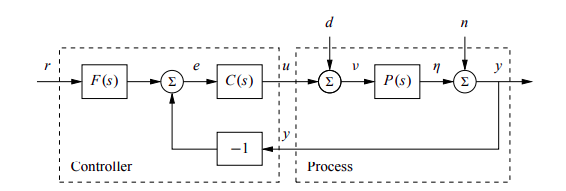
\includegraphics[width=0.8\textwidth]{images/feedback.png}
\end{center}
\caption{A general feedback system taken from \cite{scientist}}
\label{fig:feedback}
\end{figure}

\noindent We are actually interested in having the relation between the input of the system $r$ and the control input $u$ in order to have an idea of how the saturation is reached since we assume our $P(s)$ known (we can identify all the parameters of our DC motors).
\begin{equation}
  CS(jw) = \frac{C(jw)}{1+C(jw)P(jw)}
\end{equation}

\section{Noise Sensitivity Responses}

In our case let's consider a basic position control architecture for a simplified motor model (only the mechanical part is considered) as depicted in Fig \ref{fig:control}

\begin{figure}[H]
\begin{center}
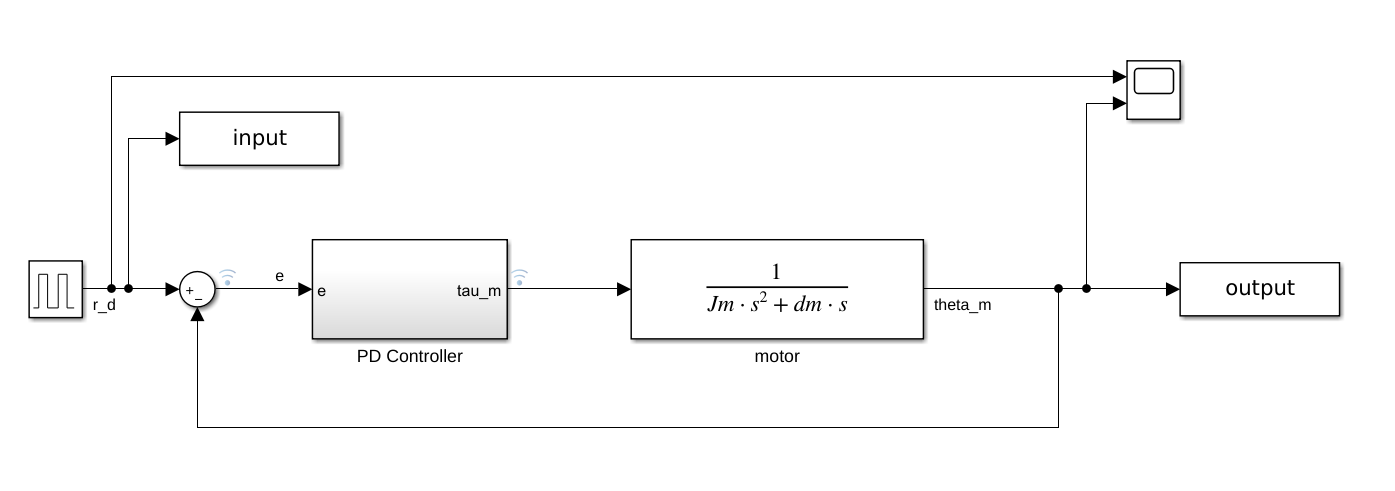
\includegraphics[width=1\textwidth]{images/position.png}
\end{center}
\caption{Simulink model of a basic position control architecture}
\label{fig:control}
\end{figure}

\noindent Our aim is to replace the input with a correctly scaled sinusoidal function that guarantees that motor saturation is not exceeded during the experiment. The PD controller can be tuned as you prefer and the motor inertia $Jm$ and motor damping $dm$ are assumed to be known. 

\bigskip
\noindent The basic idea is to use the $CS(jw)$ function to figure out at which frequency based on the reference signal we start having a gain that is above 1 meaning that we are asking more to the physical motor. In fact in this case we are sending more current to the motor that might be close to the saturation

\bigskip
\noindent In table \ref{tab:motors} different values for physical motors are reported and we be used to evaluate our approach.

\begin{table}[H]
  \begin{tabular}{ |p{6.5cm}||p{4cm}|p{4cm}| }
  \hline
  Motor& dm & jm  \\
  \hline
  SVM linear           &0.813333&   0.821697\\
  SVM poly             &0.820000&   0.826573\\
  \hline
\end{tabular}
\caption{Different motors value identified}
\label{tab:motors}
\end{table}

In Fig. \ref{fig:responses} the bode plot of the noise sensitivity function is reported

\begin{figure}[H]
\begin{center}
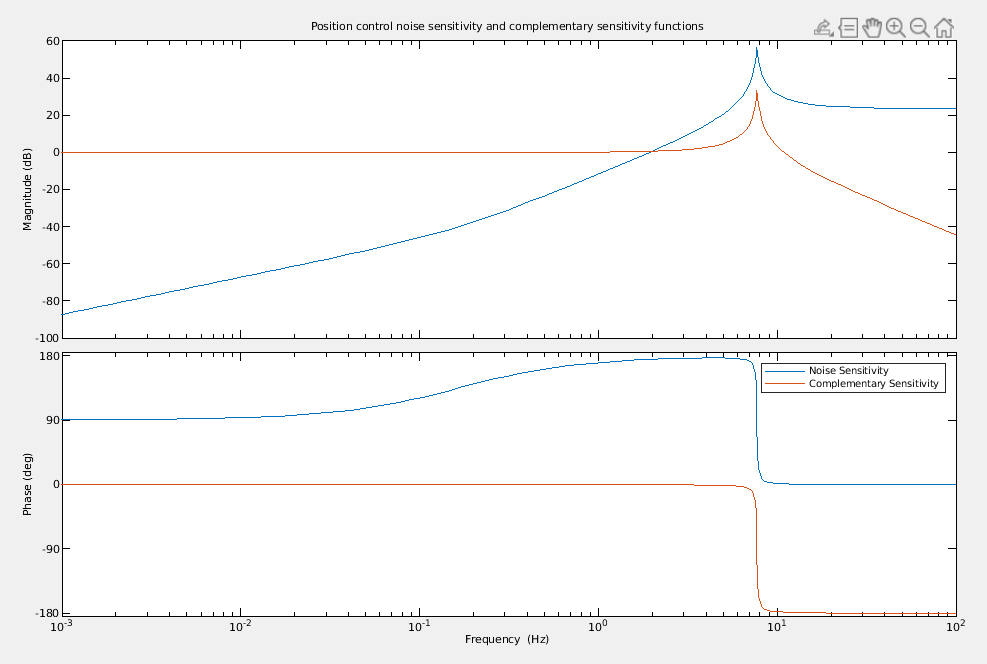
\includegraphics[width=1.0\textwidth]{images/responses.png}
\end{center}
\caption{Bode plot of the position controller of the complementary sensitivity function and noise sensitivity function}
\label{fig:responses}
\end{figure}


\begin{figure}[H]
\begin{center}
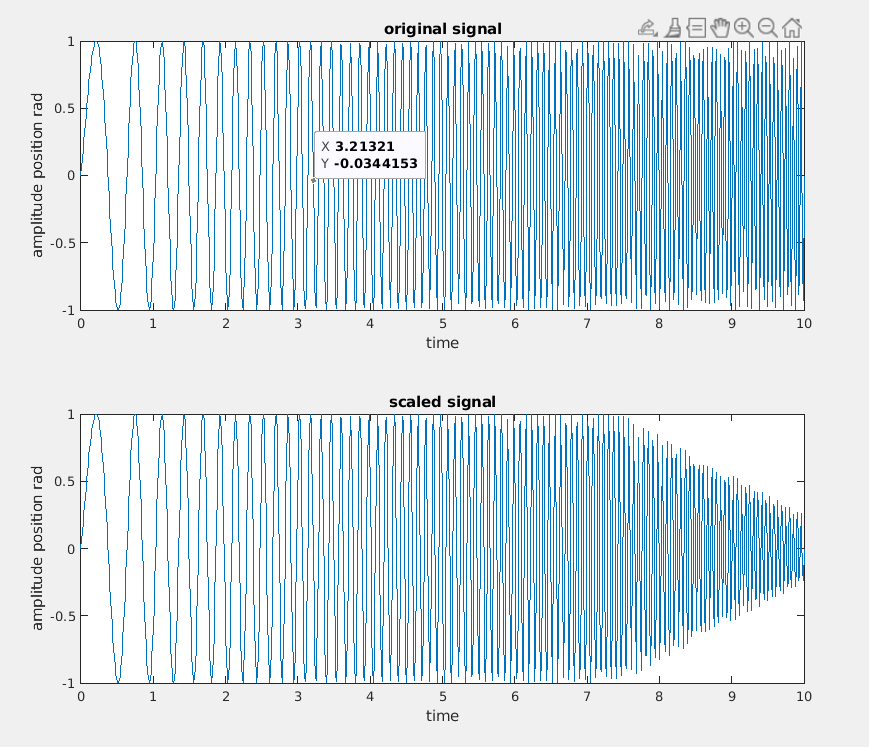
\includegraphics[width=0.9\textwidth]{images/signal.png}
\end{center}
\caption{Original vs scaled signal at a cutoff frequency of around 7.5Hz}
\label{fig:signal}
\end{figure}
  

\begin{thebibliography}{9}

\bibitem{Forecast}
Forecast Project https://eurobench2020.eu/developing-the-framework/force-control-algorithms-testbench-forecast/

\bibitem{scientist}
Karl Johan Astrom, Richard M. Murray Feedback Systems An Introduction for Scientists and Engineers
\end{thebibliography}

\end{document}


